\documentclass[12pt]{amsart}
\usepackage{geometry}
\geometry{margin=0pt, top=20pt, bottom=20pt, left=20pt, right=20pt}
\usepackage{helvet}
\renewcommand{\familydefault}{\sfdefault}
\usepackage{algtop}
\usepackage[all, cmtip]{xy}
\usepackage{caption}
\usepackage{graphicx}
\usepackage{mathtools}
\usepackage[T1]{fontenc}
\usepackage[utf8]{inputenc}
\AtBeginDocument{\Large}

\usepackage{tikz}
\usetikzlibrary{arrows.meta}
\usetikzlibrary{calc}

% Shared numbering between equation and theorem counters
\makeatletter
    \let\c@equation\c@theorem
\makeatother
\numberwithin{equation}{section}

% ---- Custom commands from main.tex ----
\newcommand{\AF}{\mathrm{AF}}
\newcommand{\ESS}[1]{\prescript{#1\!}{}{E}}
\newcommand{\ZESS}[1]{\prescript{#1\!}{}{Z}}
\newcommand{\BESS}[1]{\prescript{#1\!}{}{B}}
\newcommand{\SynSS}{\prescript{\mathrm{syn}\!}{}{E}}
\newcommand{\HF}{\mathrm{H}\bF_2}

% TikZ colors
\definecolor{lightgray}{RGB}{200,200,200}
\definecolor{llgray}{RGB}{235,235,235}

% TikZ helpers
\newcommand{\tikzgrid}[4]{%
    \foreach \x in {#1,...,#2} {
        \draw[black!20] (\x-0.5, #3-0.5) -- (\x-0.5, #4-0.5);
    }
    \foreach \y in {#3,...,#4} {
        \draw[black!20] (#1-0.5, \y-0.5) -- (#2-0.5, \y-0.5);
    }
}
\newcommand{\drawarrow}{\draw[-{Stealth[length=1.5mm]}, shorten >=(0.08cm)]}

% Dummy labels for cross-references from other sections
\newcommand{\phantomlabels}{%
    \label{sec:e6be737c}%
    \label{nota:6fb333a2}%
    \label{prop:30e8b746}%
    \label{cor:aed3d1a4}%
    \label{cor:166dc180}%
    \label{cor:290d35ce}%
    \label{prop:59f111f}%
    \label{exam:synEinfty}%
}

\title{Section 4: Synthetic Extensions (Standalone)}
\author{}
\date{}

\begin{document}
\maketitle

% Register phantom labels so \ref{...} resolves without warnings
\phantomlabels

\section{Synthetic Extensions} \label{sec:synext}
%The extension spectral sequence introduced in Section \ref{sec:e6be737c} can be generalized for $\HF$-synthetic spectra. Consider a map $f: X\to Y$ between two connective finite $\HF$-synthetic spectra\footnote{In our solution to the Kervaire invariant problem, we only consider finite synthetic spectra. However, the arguments in this section apply to any synthetic spectra for which the synthetic Adams spectral sequence strongly converges.}. By filtering$$0\to \pi_{*,*}X\fto{\pi_{*,*}f} \pi_{*,*}Y\to 0$$
%using the Adams filtration, we obtain an $f$-extension spectral sequence:
%$$\ESS{f}_0^{s,t,w} \cong E_\infty^{s,t,w}(X) \oplus E_\infty^{s,t,w}(Y) \Longrightarrow \Ker(\pi_{*,*}f)\oplus \Coker(\pi_{*,*}f)$$
%with differential
%$$d_n^f: \ZESS{f}_{n-1}^{s,t,w}(X)\to E_\infty^{s+n,t+n,w}(Y)/\BESS{f}_{n-1}^{s+n,t+n,w}(Y)$$
%where $\ZESS{f}_*^{*,*,*}$ and $\BESS{f}_*^{*,*,*}$ are  analogous to the notations in Notation \ref{nota:6fb333a2}, with the addition of an extra degree.

%In fact all the definitions and results in Section \ref{sec:e6be737c} remain valid in this synthetic setting, provided we include the extra weight degree in addition to the topological degree and ensure that all maps also preserve the weight degree. For convenience, we will not restate these results here but will occasionally refer to them and apply their synthetic versions when needed.
\paragraph{}for any map $f:X\rightarrow Y$ of synthetic spectra, we have the induced mophism of converging spectra. The resulting extension spectral sequence is denoted by the ess of $f$.


\subsection{lambda extension}
\begin{notation} \label{not:deltaandrho}
There are certain special maps between synthetic spectra that we want to consider. For any $n<m\le \infty$ and a spectrum $X$, we have the following  distinguished triangles of $\HF$-synthetic spectra
$$\Sus^{0,-n}\nu X/\lambda^{m-n}\fto{\lambda^n} \nu X/\lambda^m\fto{~\rho_{n,m}~} \nu X/\lambda^n\fto{~\delta_{n,m}~} \Sus^{1,-n}\nu X/\lambda^{m-n}.$$
We simply write $\rho=\rho_{n,m}$, $\delta=\delta_{n,m}$ by abuse of notation if $n,m$ is understood in the context.
When $m=\infty$, this sequence is interpreted  as
$$\Sus^{0,-n}\nu X\fto{\lambda^n} \nu X\fto{~\rho~} \nu X/\lambda^n\fto{~\delta~} \Sus^{1,-n}\nu X.$$

%Many arguments for finite $m$ implies the corresponding statement when $m=\infty$ because of
%$$\nu X=\varprojlim_{m} \nu X/\lambda^m$$as shown in \cite[Proposition A.13]{BHS}.

%We also note that our grading for the triangulation translation functor is smashing with $S^{1,0}$, which is consistent with \cite[Appendix A]{BHS} but is different from \cite[Section 7]{BurklundXu}.
\end{notation}

%First we show that there are no $\lambda^n$ or $\rho$-hidden extensions.

\begin{proposition}\label{prop:9770ae6e}
The only nonzero differentials in the extension spectral sequences for the maps $\lambda^n$ and $\rho$ from Notation~\ref{not:deltaandrho} are the $d_0$'s:
$$d^{\lambda^n}_0=\lambda^n \ \text{and} \ d^{\rho}_0=\rho.$$
As a result, these $d_0$'s have no crossings.
\end{proposition}
\begin{proof}
    First, we show that the the following sequence is exact in the middle:
    \begin{equation}\label{eq:d8ee7ffe}
        \scalebox{1}{$E_\infty^{s,t,w}(\Sus^{0,-n}\nu X/\lambda^{m-n})\fto{\lambda^n} E_\infty^{s,t,w}(\nu X/\lambda^{m})\fto{\rho} E_\infty^{s,t,w}(\nu X/\lambda^{n})$}.
    \end{equation}
    We apply Proposition \ref{prop:30e8b746} and prove this case by case.

    When $t-w<0$ or $t-w\ge m$, the middle group $E_\infty^{s,t,w}(\nu X/\lambda^{m}) = 0$, so the sequence is exact in the middle.

    When $0\le t-w<n$, the sequence is isomorphic to
    $$0\to Z^{s,t}_{m-t+w}(X)/B^{s,t}_{1+t-w}(X)\to Z^{s,t}_{n-t+w}(X)/B^{s,t}_{1+t-w}(X)$$
    which is exact in the middle because the second map is clearly injective.

    When $n\le t-w<m$, the sequence is isomorphic to
    $$Z^{s,t}_{m-t+w}(X)/B^{s,t}_{1+t-w-n}(X)\to Z^{s,t}_{m-t+w}(X)/B^{s,t}_{1+t-w}(X)\to 0$$
    which is exact in the middle because the first map is clearly surjective.

    Thus, we have shown that (\ref{eq:d8ee7ffe}) is always exact in the middle. Combined with Corollary \ref{cor:aed3d1a4} we conclude that all $d^{\lambda^n}_i$, $d^{\rho}_i$ are trivial for $i>0$.
\end{proof}

\begin{remark}
    From the proof above, we see that in (\ref{eq:d8ee7ffe}), $\lambda^n$ is surjective or trivial, while $\rho$ is injective or trivial.
\end{remark}

\subsection{delta extension}

\paragraph{}
However, the $\delta$-extension spectral sequence for
$$\delta:\nu X/\lambda^n\to \Sus^{1,-n}\nu X/\lambda^{m-n}$$
is more complicated, as it encodes classical Adams differentials $d_2$ through $d_m$.

\begin{remark}
    For the convenience of readers to check gradings, whenever we write
    $$d_{n}^{f}(x)=\lambda^k y$$
    for $f: \Sus^{m,w} \nu X\to \nu Y$,
    $x\in E_\infty^{s_1,t_1,w_1}(\nu X)$ and
    $y\in E_\infty^{s_2,t_2,w_2}(\nu Y)$,
    the following conditions must hold:
    $$s_2=s_1+n, \ t_2-s_2=t_1-s_1+m, \ \text{and} \ w_2=w_1+w.$$
\end{remark}

\begin{proposition}\label{prop:6de7d130}
    Suppose in the classical Adams spectral sequence of $X$ we have $d_r(x)=y$, where $x\in Z_{r-1}^{s,t}(X)$ and $y\in Z_\infty^{s+r,t+r-1}(X)$. Consider the map
    $$\delta:\nu X/\lambda^n\to \Sus^{1,-n}\nu X/\lambda^{m-n}.$$
    \begin{enumerate}
        \item If $r\ge n+1$, then we view $x$ as an element of
        $$E_\infty^{s,t,t}(\nu X/\lambda^n)\iso Z_n^{s,t}(X),$$
        and $\lambda^{r-n-1} y$ as an element of
        $$E_\infty^{s+r,t+r-1, t+n}(\nu X/\lambda^{m-n})\iso Z_{m-r+1}^{s+r,t+r-1}(X)/B_{r-n}^{s+r,t+r-1}(X).$$
        We then have
        $$d^{\delta}_r(x)=\lambda^{r-n-1}y,$$
        which is trivial if $r>m$.
        \item If $r<n+1$, then we view $\lambda^{n+1-r}x$ as an element of
        $$E_\infty^{s,t,t-n-1+r}(\nu X/\lambda^n)\iso Z^{s,t}_{r-1}(X)/B^{s,t}_{n+2-r}(X),$$
        and $y$ as an element of
        $$E_\infty^{s+r,t+r-1, t+r-1}(\nu X)\iso Z_\infty^{s+r,t+r-1}(X).$$
        In this case, we have
        $$d^{\delta}_r(\lambda^{n+1-r}x)=y.$$
    \end{enumerate}
\end{proposition}
\begin{proof}
    Since $\delta=\delta_{n,m}$ is the composition of $\rho$ and $\delta_{n,\infty}$ as the following
     $$\xymatrix{
    \nu X/\lambda^n\ar[d]_-{\delta_{n,\infty}} \ar[rd]^{\delta_{n,m}} & \\
    \Sus^{1,-n}\nu X\ar[r]_-{\rho} & \Sus^{1,-n}\nu X/\lambda^{m-n}
    }$$
    it suffices to prove the case when $m=\infty$ by Corollary \ref{cor:290d35ce}. In the rest of the proof we will write $\delta_n=\delta_{n,\infty}$.

    First, we prove by induction on $n$ that
    \begin{equation}\label{eq:24e1e3f6}
        d^{\delta_n}_r(x)\equiv \lambda^{r-n-1}y\mod B_{r-1}^{s+r,t+r-1}(X)
    \end{equation}
    when $r\ge n+1$, and
    \begin{equation}\label{eq:2f8e024e}
        d^{\delta_n}_r(\lambda^{n+1-r}x)\equiv y\mod B_{r-1}^{s+r,t+r-1}(X)
    \end{equation}
    when $r\le n+1$. (These two expressions coincide when $r=n+1$.) For $n=1$, the claim holds since the $\tau$-Bockstein spectral sequence is isomorphic to the classical Adams spectral sequence. Now, assume $n\ge 2$ and the claim holds for $n-1$.

    Consider the following commutative diagram.
    $$\xymatrix{
        \Sus^{0,-1}\nu X/\lambda^{n-1} \ar[rd]_-{\delta_{n-1}} \ar[r]^-\lambda &  \nu X/\lambda^{n}\ar[d]^-{\delta_{n}}\\
        & \Sus^{1,-n}\nu X\\
    }$$
    By Corollary \ref{cor:166dc180}, if $r\le n$, we have
    $$d^{\delta_{n}}_r(\lambda^{n+1-r}x)=d^{\delta_{n-1}}_r(\lambda^{n-r}x)\equiv y\mod B_{r-1}^{s+r,t+r-1}(X).$$
    If $r\ge n+1$, $x$ can be viewed as an element of the $E_\infty$-pages of $\nu X/\lambda^{n-1}$ or $\nu X/\lambda^n$. We then have
    $$\lambda d^{\delta_{n}}_r(x)=d^{\delta_{n}}_r(\lambda x)=d^{\delta_{n-1}}_r(x)\equiv \lambda^{r-n}y \mod B_{r-1}^{s+r,t+r-1}(X)$$
    which implies
    $$d^{\delta_{n}}_r(x)\equiv\lambda^{r-n-1}y\mod B_{r-1}^{s+r,t+r-1}(X),$$
    since $r-n+1\le r-1$ and hence the indeterminacy $B_{r-n+1}$ introduced by dividing $\lambda$ is contained in $B_{r-1}$. The induction for (\ref{eq:24e1e3f6}) and (\ref{eq:2f8e024e}) is now complete.

    We will show that
    $B_{r-1}^{s+r,t+r-1}(X)$ in both equations are actually equal to the sum of images of $d^{\delta_{n}}_0$ through $d^{\delta_{n}}_{r-1}$.
    Consider any $y'\in B_{r-1}^{s+r,t+r-1}(X)$ and assume that $d_{r'}x'=y'$ is an essential classical Adams differential for $2\le r'\le r-1$. If $r\ge n+1$, using (\ref{eq:24e1e3f6}), we have
    $$d^{\delta_n}_{r'}(\lambda^{r-r'}x)\equiv \lambda^{r-n-1}y'\mod B_{r'-1}^{s+r,t+r-1}(X),$$
    and if $r\leq r'+1$, using (\ref{eq:2f8e024e}), we have
    $$d^{\delta_n}_{r'}(\lambda^{n+1-r'}x')\equiv y'\mod B_{r'-1}^{s+r,t+r-1}(X).$$
    Notice that the extra indeterminacy here is $B_{r'-1}$ instead of $B_{r-1}$. By induction on $r$, this shows that $B_{r-1}^{s+r,t+r-1}(X)$ equals the sum of images of $d^{\delta_{n}}_0$ through $d^{\delta_{n}}_{r-1}$.

    Therefore, we can omit $B_{r-1}^{s+r,t+r-1}(X)$ and simply write
    $$d^{\delta_n}_r(x)= \lambda^{r-n-1}y$$
    when $r\ge n+1$, and
    $$d^{\delta_n}_r(\lambda^{n+1-r}x)= y$$
    when $r\le n+1$.
\end{proof}

\begin{remark}
    The $d^{\delta}_r(x)$ we calculated in Proposition \ref{prop:6de7d130} may be inessential.
\end{remark}

\subsection{delta ess and Adams}
\begin{corollary}\label{cor:2a636737}
    For $x,y,\delta$ in Proposition \ref{prop:6de7d130} we always have
    \begin{equation}\label{eq:841425e9}
        d^{\delta}_r(\lambda^ax)=\lambda^{a+r-n-1}y
    \end{equation}
    if $0\le a\le n$ and $0\le a+r-n-1<m-n$ (the differential is trivial if $a$ exceeds this range).
\end{corollary}

\begin{remark}\label{rmk:qvoewfj}
    As indicated in the proof, the right-hand side of equation (\ref{eq:841425e9}) (considered as a subset of $Z_\infty^{s+r,t+r-1}(X)$) is a coset of
    $$B_{r-1}^{s+r,t+r-1}(X)$$
    which is the same as the value of the classical Adams differential $d_r(x)=y$. This implies that the equation (\ref{eq:841425e9}) holds and essential if and only if $d_r(x)=y$ and essential . Therefore the $\delta$-ESS encodes the same information as the classical Adams spectral sequence.
\end{remark}

\subsection{Er corssing}
\begin{definition} \label{def:classicalcrossdiff}
    Suppose $r\ge n+1$ and $d_r(x)=y$, where
    $$x\in E_2^{s,t}(X), \hspace{0.5cm} y\in E_2^{s+r,t+r-1}(X).$$
    A crossing of $d_r(x)=y$ on the $E_{n+1}$-page refers to an essential Adams differential
    $$d_{r-a-b}(x^\prime)=y^\prime,$$
    where
    $$x^\prime\in E_2^{s+a,t+a}(X), \hspace{.5cm} y^\prime\in E_2^{s+r-b,t+r-b-1}(X),$$
    with $0<a\le n-1$ and $0\le b\le r-n-1$. See Figure \ref{fig:f5eae42a}.
\end{definition}

\begin{remark}
    The crossing defined here is opposite to crossings in Moss's theorem.
\end{remark}
\begin{figure}[h]
\centering
\scalebox{0.8}{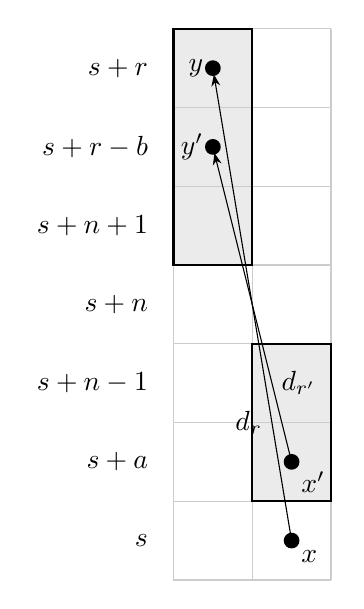
\begin{tikzpicture}
    % Draw grid
    \fill[llgray] (1-0.5, 1-0.5) rectangle ++(1, 2);
    \fill[llgray] (0-0.5, 4-0.5) rectangle ++(1, 3);
    \tikzgrid{0}{2}{0}{7}
    \draw[thick] (1-0.5, 1-0.5) rectangle ++(1, 2);
    \draw[thick] (0-0.5, 4-0.5) rectangle ++(1, 3);

    % Draw bullets
    \coordinate (x) at (1, 0);
    \coordinate (y) at (0, 6);
    \coordinate (x1) at (1, 1);
    \coordinate (y1) at (0, 5);

    \fill (x) circle (0.1) node[below right] {$x~$};
    \fill (x1) circle (0.1) node[below right] {$x'$};
    \fill (y) circle (0.1) node[left] {$y$};
    \fill (y1) circle (0.1) node[left] {$y'$};

    % Draw differentials
    \drawarrow (x) -- (y) node[near start, left] {$d_r$};
    \drawarrow (x1) -- (y1) node[near start, right] {$d_{r'}$};

    \node[anchor=east] at (-.7, 0) {$s$};
    \node[anchor=east] at (-.7, 1) {$s+a$};
    \node[anchor=east] at (-.7, 2) {$s+n-1$};
    \node[anchor=east] at (-.7, 3) {$s+n$};
    \node[anchor=east] at (-.7, 4) {$s+n+1$};
    \node[anchor=east] at (-.7, 5) {$s+r-b$};
    \node[anchor=east] at (-.7, 6) {$s+r$};
\end{tikzpicture}}
\caption{A crossing of $d_r(x)=y$ on the $E_{n+1}$-page}\label{fig:f5eae42a}
\end{figure}


\subsection{comparison of crossing}
The emphasis on a crossing occurring ``on the $E_{n+1}$-page" in Definition~\ref{def:classicalcrossdiff} may seem counter-intuitive. However, this is clarified in Proposition~\ref{prop:cross-dr-En} and Example~\ref{exam:classcrossdiff} that follow.

\begin{proposition}\label{prop:cross-dr-En}
    The Adams differential $d_r(x)=y$ has a crossing on the $E_{n+1}$-page if and only if the corresponding $\delta_n$-extension
    $$d^{\delta_n}_r(x)=\lambda^{r-n-1}y$$
    for
    $$\delta_{n}:\nu X/\lambda^{n}\to \Sus^{1,-n}\nu X$$
    has a crossing.
\end{proposition}
\begin{proof}
    By Propositions \ref{prop:30e8b746}, \ref{prop:59f111f} and \ref{prop:6de7d130}, a crossing of $d^{\delta_n}_r(x)=\lambda^{r-n-1}y$ takes the form
    $$d^{\delta_n}_{r-a-b}(\lambda^a x')=\lambda^{r-n-1-b}y',$$
    where $0<a\le n-1$, $0\le b\le r-n-1$,
    $$\lambda^a x'\in E_\infty^{s+a,t+a,t}(\nu X/\lambda^n)\iso Z_{n-a}^{s+a,t+a}(X)/B_{1+a}^{s+a,t+a}(X),$$
    and
    $$y'\in E_\infty^{s+r-b, t+r-b-1}(\nu X).$$
    By Corollary \ref{cor:2a636737}, we see that this crossing corresponds to the classical Adams differential
    $$d_{r-a-b}(x')=y'.$$
\end{proof}

\begin{remark} \label{nocrossE2}
    From Definition~\ref{def:classicalcrossdiff}, it immediately follows that there are no crossings of any differential on the $E_2$-page, as this would require $0< a \le n-1 = 0$. According to Proposition~\ref{prop:cross-dr-En}, this reflects the fact that $\delta_1$-extensions have no crossings for degree reasons.
\end{remark}

\begin{remark}
    When $d_r^{\delta_n}(x) = \lambda^{r-n-1}y$ has no crossing, then 
    $d_r^{\delta_n}(\lambda^a)(x) = \lambda^?y$ also has no crossing.
\end{remark}


\end{document}
